\documentclass[12pt, twoside]{article}
\usepackage[francais]{babel}
\usepackage[T1]{fontenc}
\usepackage[latin1]{inputenc}
\usepackage[left=7mm, right=7mm, top=7mm, bottom=7mm]{geometry}
\usepackage{float}
\usepackage{graphicx}
\usepackage{array}
\usepackage{multirow}
\usepackage{amsmath,amssymb,mathrsfs} 
\usepackage{soul}
\usepackage{textcomp}
\usepackage{eurosym}
 \usepackage{variations}
\usepackage{tabvar}

\begin{document}

\ul{\textbf{Exercice 4 (remani�):}}
Voici trois expressions:
  \begin{center}
$A= 12 - \dfrac{0,9 \times 30}{3}$ \qquad \qquad $B=\dfrac{12-5 \times 2}{15+2,5
\times 2}$ \qquad \qquad $C=8 \times 7-3 \times \dfrac{24 \div 3+8}{200 \times
0,02}$
\end{center}

\begin{enumerate}
  \item Calculer, � la main, chacune des expressions $A$, $B$ et $C$. 
  \item Ecrire une s�quence de touches permettant de calculer chacune d'entre
  elles avec la calculatrice.
  \item V�rifier alors avec la calculatrice les r�sultats obtenus � la premi�re
  question.
\end{enumerate}

\bigskip


\ul{\textbf{Exercice 6:}} Recopier les expressions suivantes en supprimant les
parenth�ses inutiles puis effectuer les calculs.

\begin{center}
$A= 18-(3 \times 5)$ \qquad $B=8 \times (27+3)$ \qquad $C= (3 \times 8)
-(15-12)$ \qquad $D=3 \times (5 \times 9)$.
\end{center}

\bigskip 

\begin{center}
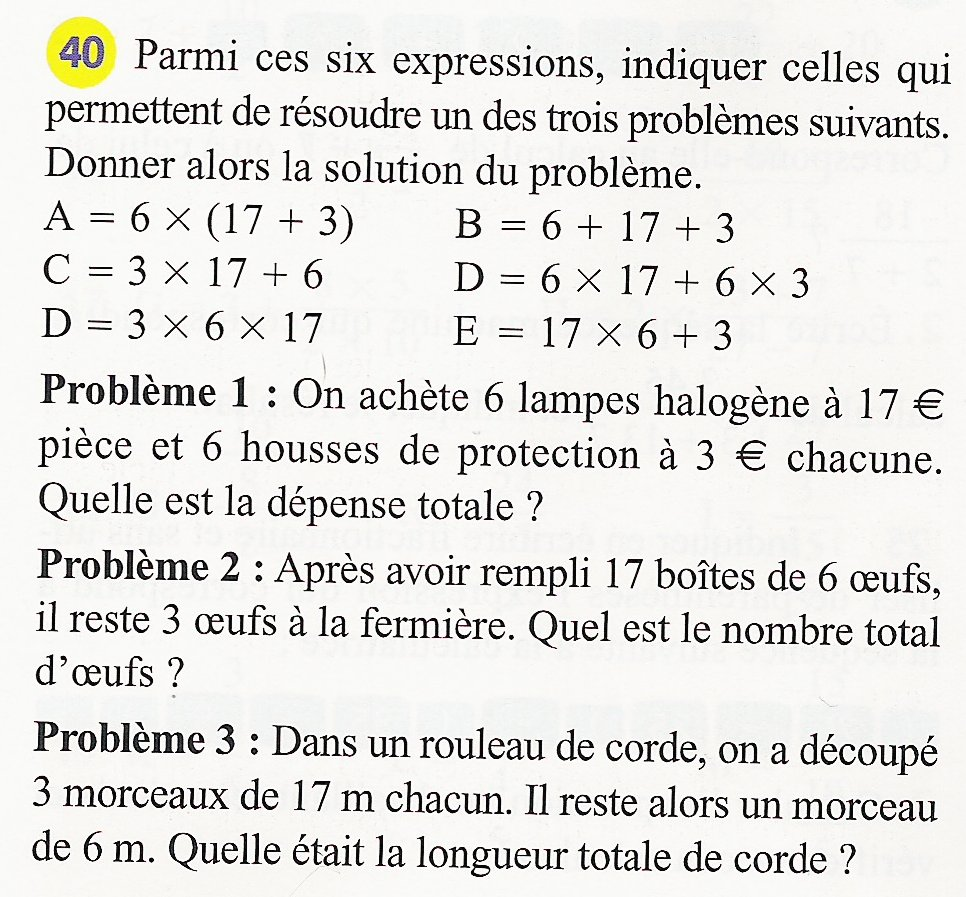
\includegraphics[width=8cm]{image/pb.jpg}
\end{center}

\bigskip

\ul{\textbf{Exercice 7:}} Recopier les expressions suivantes en ajoutant les
signes $\times$ qui sont sous-entendus.

\begin{center}
$A=2 \pi r$ \qquad $B=3(a-4)$ \qquad $C=(a+15)(b-3)$ \qquad $D=5b+2a$
\end{center}

\bigskip

\ul{\textbf{Exercice 8:}} Recopier les expressions suivantes en supprimant le
signe $\times$ quand c'est possible (on ne demande pas d'effectuer les calculs).


\begin{tabular}{cc}
\begin{minipage}{9cm}
$A=8 \times a$

$B=4,2 \times 5$

$C=8 \times (17,3 + a)$

$D=(20,3-2) \times (7,8 -6)$

\end{minipage}
&
\begin{minipage}{9cm}
$E=2 \times 3+6$

$F=6 \times 6 \times 6$

$G=8 \times 8$

$H=4 \times  2 \times k$

$I=x \times y \times z$

\end{minipage}
\end{tabular}

\bigskip

\ul{\textbf{Exercice 9:}} Calculer mentalement: $5^{2}$; \qquad $3^{2}$; \qquad
$2^{3}$; \qquad $0^{2}$; \qquad $3^{3}$;
\end{document}
